
%(BEGIN_QUESTION)
% Copyright 2012, Tony R. Kuphaldt, released under the Creative Commons Attribution License (v 1.0)
% This means you may do almost anything with this work of mine, so long as you give me proper credit

Three-phase AC induction motors respond differently to the loss of one phase, depending on whether they are internally wye- or delta-connected:

$$\includegraphics[width=15.5cm]{i00967x01.eps}$$

Which of these two motor designs will fare better in the event of a phase loss such as the open fault in phase C shown above, and why?

\underbar{file i00967}
%(END_QUESTION)





%(BEGIN_ANSWER)

The delta-connected motor will fare better, because it will still generate a polyphase (truly rotating) magnetic field, whereas the wye-connected motor will only generate an oscillating magnetic field.  Also, the voltage across each phase winding of the delta-connected motor will remain the same as the line voltage, while the voltage across each phase winding of the wye-connected motor will decrease from what it was previous to the fault.
 
If the motors' mechanical loads are sufficiently light, both motors will continue to rotate.  However, the delta-connected motor will have a greater torque capacity in this phase-loss condition than the wye-connected motor due to the fact that its rotating magnetic field still maintains a definite direction of rotation and also that each of its phase windings receives the same (full) voltage as previously.

\vskip 10pt

If these consequences are not clear for you to see, you might wish to apply the problem-solving technique of {\it adding quantitative values} to the problem.  Assign a line voltage (e.g. 480 VAC) to the incoming three-phase power conductors A, B, and C.  Then, analyze the voltages at each phase winding of each motor before the fault versus after the fault.  You may also calculate the {\it phase angle} for each of these winding voltages to see that the delta-connected motor still has three 120$^{o}$-shifted voltages powering it, while the wye-connected motor only has one voltage (single phase) powering it.

%(END_ANSWER)





%(BEGIN_NOTES)


%INDEX% Electronics review: 3-phase voltage/current/power calculation

%(END_NOTES)


